%\begin{savequote}[8cm]
%\textlatin{Cor animalium, fundamentum e\longs t vitæ, princeps omnium, Microco\longs mi Sol, a quo omnis vegetatio dependet, vigor omnis \& robur emanat.}
%
%The heart of animals is the foundation of their life, the sovereign of everything within them, the sun of their microcosm, that upon which all growth depends, from which all power proceeds.
%  \qauthor{--- William Harvey \cite{harvey_exercitatio_1628}}
%\end{savequote}

\chapter{\label{app:1-basics}General plasma physics}

\minitoc
% TODO: Add simulation parameters

\section{Lorentz transformations of electromagnetic fields}\label{sec:app_lorentzEM}
The Lorentz transformations for electromagnetic field components parallel, $\parallel$, and perpendicular, $\perp$, to a frame of reference boost of velocity $\mathbf{v}$ are \cite{steaneRelativityMadeRelatively2012}
\begin{equation}\label{eq:app-maxwell_transformation}
	\mathbf{E}'_\parallel = \mathbf{E}_\parallel,
\end{equation}
\begin{equation}
	\mathbf{B}'_\parallel = \mathbf{B}_\parallel,
\end{equation}
\begin{equation}
	\mathbf{E}'_\perp = \gamma_\mathbf{v}(\mathbf{E}_\perp + \mathbf{v} \times \mathbf{B}),
\end{equation}
\begin{equation}
	\mathbf{B}'_\perp = \gamma_\mathbf{v}(\mathbf{B}_\perp - \mathbf{v} \times \mathbf{E}/c^2).
\end{equation}

\section{The headlight effect}\label{sec:app_headlight}
The headlight effect describes the beaming of an isotropically emitting source travelling at some velocity relative to an observer. Consider the geometry of figure \ref{fig:zvp_ablatingfront} with the source (the laser pulse) travelling at an angle $2\theta$ to the observer (in this case, the ablating front). A photon with energy $E$ emitted from the rest frame of the source (the laboratory frame in this case) has a 4-momentum
\begin{equation}
	\mathbf{P}_\mu = \left(\frac{E}{c},\frac{E}{c}\cos{2\theta},\frac{E}{c}\sin{2\theta}\right).
\end{equation}
As the interaction geometry is confined to a 2D plane,  the $z$-component can be safely neglected. Applying the lorentz boost of equation \ref{eq:zvp_lorentz},
\begin{equation}
	\begin{split}
		\frac{E'}{c} = \gamma \left( \frac{E}{c} - \beta \frac{E}{c}\cos{2\theta}\right) \\
		\frac{E'}{c}\cos{2\theta'} = \gamma \left( \frac{E}{c}\cos{2\theta} - \beta \frac{E}{c}\right).
	\end{split}
\end{equation}
Solving these equations for the angle in the boosted frame,
\begin{equation}
	\cos{2\theta'} = \frac{\cos{2\theta} - \beta}{1-\beta\cos{2\theta}}.
\end{equation}

\section{\label{app:1-basics-transverse_emittance}Geometric transverse emittance}
A beam\footnote{In this section it is electron beams and not bunches that a referred to to demonstrate the generality of these concepts.} of particles is fully described by its six-dimensional particle phase space distribution
\begin{equation}
	\rho(\mathbf{x}, \mathbf{p}) = \rho(x,p_x,y,p_y,z,p_z),
\end{equation}
where $\mathbf{p} = p_x \hat{\mathbf{x}} +  p_y \hat{\mathbf{y}} +  p_z \hat{\mathbf{z}}$ is the canonical momentum \cite{mcdonaldMethodsEmittanceMeasurement1989}. Under the Hamilton formalism, for ideal conditions, the six-dimensional volume of the beam in this space, termed the \textit{emittance}, arises as a conserved quantity and is therefore a useful quantity to describe the beam quality. 
(something to do with it affecting the ability to focus the beam?? check the papers)
It is useful to rotate the coordinate system so as to align with the beam's propagation. The distribution can be written as
\begin{equation}
	\rho(\mathbf{x'}, \mathbf{p'})  = \rho(x_\mathrm{L},p_\mathrm{L},x_\mathrm{T},p_\mathrm{T},x_\mathrm{T'},p_\mathrm{T'}),
\end{equation}
where L is longitudinal to the beam's propagation direction, and T and T$'$ are two orthogonal directions transverse to the beam's propagation. Where discussed in this thesis, T$'$ will unanimously refer to the $z$-direction, that is, the additional direction in 3D simulations, all such simulations are designed such that the $z$-direction is transverse to the beam propagation direction.

Recording a six-dimensional phase space in experiment is impossible while in simulations it is almost prohibitively costly in terms of data storage. Hence, it is common practice to project the distribution onto three orthogonal sub-spaces corresponding to each spatial axis, L, T and T$'$ and compute the area on each. Note that since the electron beam is ultra-relativistic, all electrons propagate at approximately c and therefore it is the transverse and not the longitudinal emittance that describes the beam's quality. As a particle beam does not typically exist with well-defined borders, the area used to describe the emittance is restricted to an ellipse containing only the high-density core of the distribution. For a subspace $i$, where $i = $ T or T$'$, Floettmann \textit{et al} \cite{floettmannBasicFeaturesBeam2003} derive the \textit{transverse normalised emittance} as
\begin{equation}\label{eq:app_epsilon_n}
	\epsilon^i_\mathrm{n,rms} = \frac{1}{m_\mathrm{e}c} \sqrt{\langle x^2_i\rangle\langle p^2_i\rangle - \langle x_ip_i\rangle^2},
\end{equation}
where $\langle\rangle$ is the second central moment of the particle distribution,
\begin{equation}
	\langle ab \rangle = \frac{\int ab\rho(\mathbf{x}',\mathbf{p}')dV}{\int \rho (\mathbf{x}',\mathbf{p}')dV} - \frac{\int a\rho(\mathbf{x}',\mathbf{p}')dV\int a\rho(\mathbf{x}',\mathbf{p}')dV}{(\int \rho (\mathbf{x}',\mathbf{p}')dV)^2},
\end{equation}
here $dV = \Pi_jdx_jdp_j$ for $j = $L, T, T$'$.

When working with emittances, most frequently in the literature it is the \textit{transverse geometric emittance}, $\epsilon^i_\mathrm{rms}$ that is discussed. This is a natural consequence of it being more readily accessible in experiments \cite{mcdonaldMethodsEmittanceMeasurement1989}. The geometric and normalised emittances are related via
\begin{equation}
	\epsilon^i_\mathrm{rms} = \frac{\epsilon^i_\mathrm{rms}}{\gamma \beta_\mathrm{L}},
\end{equation}
where $\gamma = 1/\sqrt{1-\beta^2}$ refers to the beam's mean energy and $\beta_\mathrm{L} \approx c$ is the ultrarelativistic beam's longitudinal speed.

The Courant-Snyder invariant which describes the ellipse that corresponds to the emittance is\footnote{Regrettably $\beta$ and $\gamma$ are the standard notations for the Twiss parameters, at all other locations in this Thesis, these parameters will refer to the standard relativistic beta and gamma factors of objects respectively.}
\begin{equation}
	\epsilon^i_\mathrm{rms}  = \gamma x_i^2 + 2\alpha x x' \beta x_i'^2,
\end{equation}
here the coordinates are $x_i$ and $x'_i = p_i/p_\mathrm{L}$ \cite{wiedemannParticleAcceleratorPhysics2015}. The Twiss parameters are
\begin{equation}
	\alpha = - \frac{\langle x_i x'_i \rangle}{	\epsilon^i_\mathrm{rms} },
\end{equation}
\begin{equation}
	\beta = \frac{\langle x_i \rangle}{	\epsilon^i_\mathrm{rms} }
\end{equation}
and
\begin{equation}
	\gamma = \frac{\langle x_i'^2 \rangle}{	\epsilon^i_\mathrm{rms} }.
\end{equation}
Thus the shape of the ellipse and the divergence of the beam can be determined. The elliptical contour defining the emittance of an ideal Gaussian phase-space distribution is given in Figure \ref{fig:emittancenormal}.
\begin{figure}
	\centering
	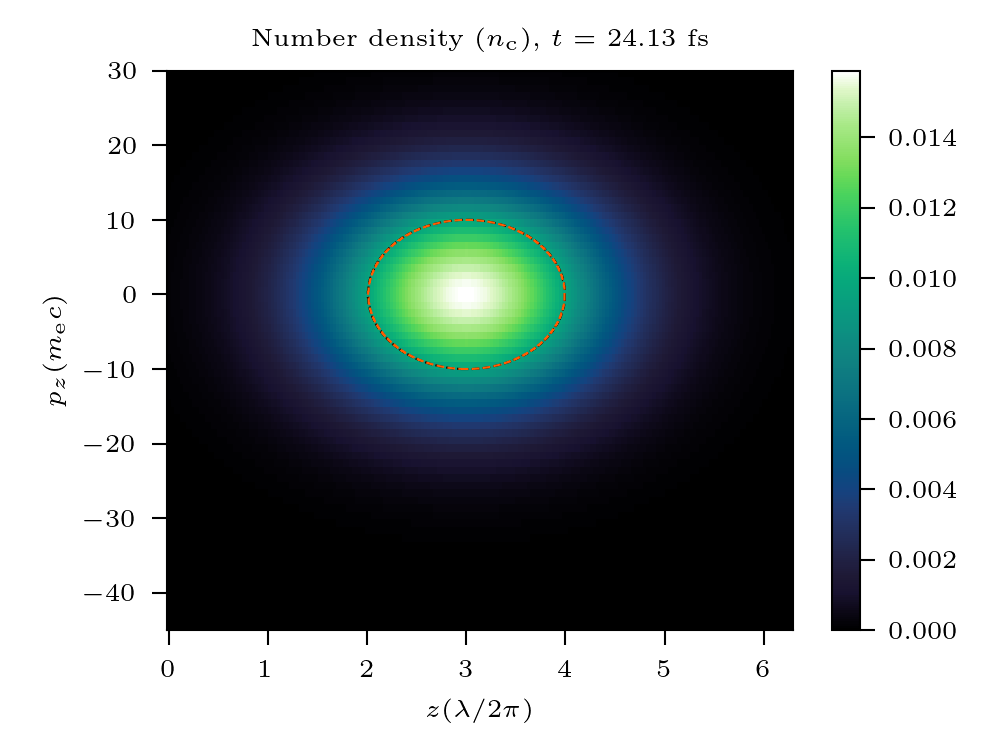
\includegraphics[width=0.7\linewidth]{figures/appendix/emittance_normal}
	\caption[Emittance calculation for an ideal Gaussian distribution in phase space.]{Emittance calculation for an ideal Gaussian distribution in phase space, $f_\mathrm{n}(z,p_z) = 1/(2\pi s_zs_{pz})\exp[-((z-m_z)^2/(2s_z^2) + (p_z-m_{pz})^2/(2s_{pz}^2))]$, centred at ($m_z$,$m_{pz}$) = (3,0) with standard deviations ($s_z$,$s_{pz}$) = (1,10).}
	\label{fig:emittancenormal}
\end{figure}
The contour is numerically calculated to contain \qty{39.4 \pm .1}{\%} of the particles, compared to 39.3 \% from theory. Here the discrepancy arises from the finite grid on which the distribution is defined.

\section{The Bourdier method}\label{sec:app-bourdier}
The Bourdier method enables the modelling of an obliquely incident laser pulse in 1D geometry \cite{bourdierObliqueIncidenceStrong1983}. While some of this section may seem trivial, it is frequently misquoted in the literature. It therefore seems of great importance to provide a full derivation.

Consider a photon incident on a plasma block at angle $\theta$ as in Figure \ref{fig:miscreferenceframesboosted1d}.
\begin{figure}
	\centering
	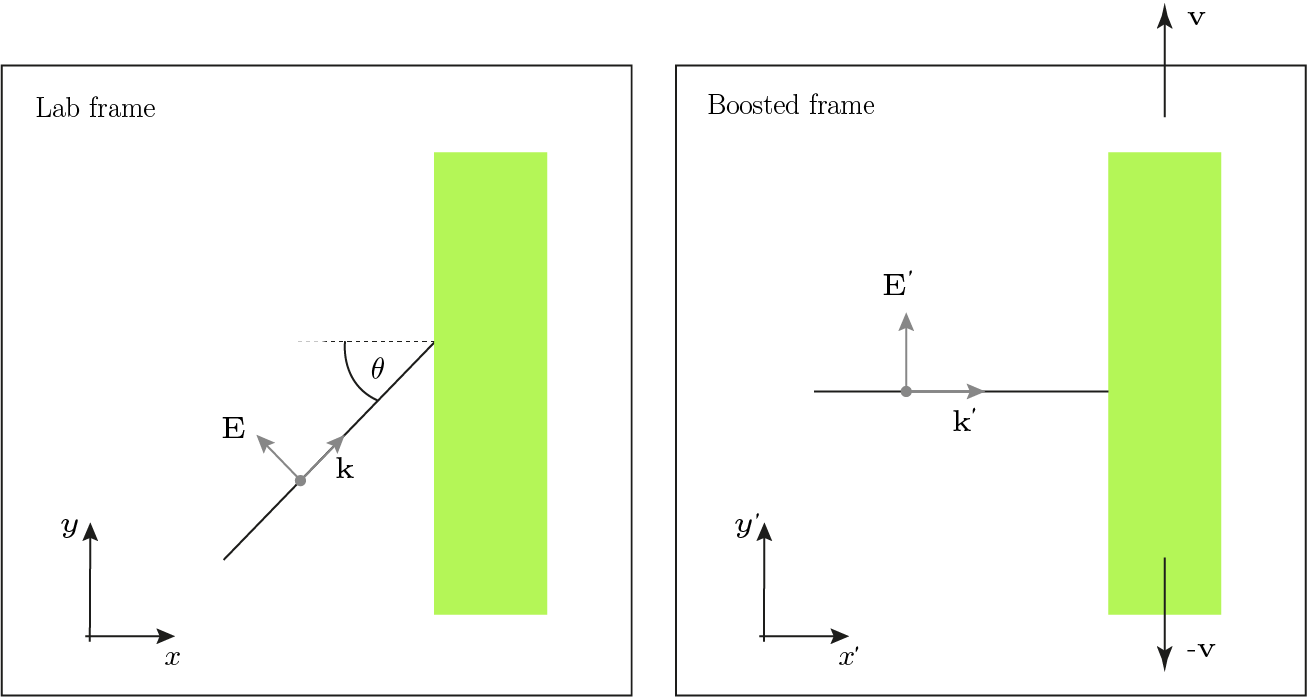
\includegraphics[width=1\linewidth]{figures/misc/misc_reference_frames_boosted_1D}
	\caption{}
	\label{fig:miscreferenceframesboosted1d}
\end{figure}
A boost is applied with velocity $\mathbf{v}$ to the laboratory frame such that the photon is normally incident on the now streaming plasma at velocity $-\mathbf{v}$. The velocity transformation for the photon's velocity, $\mathbf{u}$, parallel to the boost is
\begin{equation}
	\mathbf{u}'_\parallel = \frac{\mathbf{u}_\parallel - \mathbf{v}}{1-\mathbf{u}\cdot\mathbf{v}/c^2}.
\end{equation}
Setting  $\mathbf{u}'_\parallel = 0$, it is clear that
\begin{equation}
	\mathbf{v} = \mathbf{u}_\parallel = c\sin\theta \hat{\mathbf{y}}
\end{equation}
in this geometry and 
\begin{equation}
	\gamma_\mathbf{v} = \frac{1}{\sqrt{1-\mathbf{v}^2/c^2}}=\sec\theta.
\end{equation}
Since Snell's law is frame invariant, the photon remains normal as it propagates into the skin depth of the plasma, a frame in which the interaction reduces to a 1D problem has been successfully found for all $\theta < \pi/2$. Those familiar with the topic may wonder how this is possible considering the `ripples' that can be observed on the plasma surface for oblique incidence. The explanation for this is of course the relativity of simultaneity. 

It remains to determine how do all the relevant quantities transform as such a boost is applied. Starting with an simple one: the photon's wave four-vector is 
\begin{equation}
	\mathbf{K}^\mathrm{\mu} = \left(\frac{\omega}{c},\mathbf{k}\right)
\end{equation}
and thus the frequency transforms as
\begin{equation}
	\frac{\omega}{c} = \gamma_\mathbf{v}\left(\frac{\omega'}{c}-\frac{\mathbf{v}}{c}\cdot\mathbf{k'}\right).
\end{equation}
Since $\mathbf{v}\cdot\mathbf{k'} = 0$, 
\begin{equation}\label{eq:boost_omega}
	\omega' = \omega\cos\theta .
\end{equation}
As 
\begin{equation}
	n'_\mathrm{c} = \frac{m_\mathrm{e}(\omega')^2}{4\pi e^2},
\end{equation}
\begin{equation}\label{eq:boost_nc}
	n'_\mathrm{c} =n_\mathrm{c} \cos^2\theta ,
\end{equation}
while the plasma block will be Lorentz contracted along $\hat{\mathbf{y}}$. Hence, the number density of electrons will increase as
\begin{equation}
	n'_\mathrm{e} = \frac{n'_\mathrm{e}}{\cos\theta}
\end{equation}
leading to the perhaps unexpected
\begin{equation}
	\bar{n}'_\mathrm{e} = \frac{\bar{n}_\mathrm{e}}{\cos^3\theta}.
\end{equation}
Time is dilated 
\begin{equation}
	t' = \frac{t}{\cos\theta}.
\end{equation}

Consider now the more general case where the photon's electric field is rotated out of the $x$-$y$ plane, \textit{i.e.}
\begin{equation}
	\mathbf{E} = E_0(-\cos\phi\sin\theta,\cos\phi\cos\theta,\sin\phi)
\end{equation}
and correspondingly
\begin{equation}
	\mathbf{B} = \frac{\hat{\mathbf{k}} \times \mathbf{E}}{c}= \frac{E_0}{c}(\sin\phi\sin\theta,-\sin\phi\cos\theta,\cos\phi).
\end{equation}
The Lorentz transformations for electro-magnetic fields are
\begin{equation}
	\mathbf{E}'_\parallel = \mathbf{E}_\parallel,
\end{equation}
\begin{equation}
	\mathbf{B}'_\parallel = \mathbf{B}_\parallel,
\end{equation}
\begin{equation}
	\mathbf{E}'_\perp = \gamma_\mathbf{v}(\mathbf{E}_\perp + \mathbf{v} \times \mathbf{B}),
\end{equation}
\begin{equation}
	\mathbf{B}'_\perp = \gamma_\mathbf{v}(\mathbf{B}_\perp - \mathbf{v} \times \mathbf{E}/c^2).
\end{equation}
Using the above expressions for $\mathbf{E}_\perp$ and $\mathbf{E}_\parallel$ and transforming to the boosted frame,
\begin{equation}
	\mathbf{E}' = E_0\cos\theta (0,\cos\phi,\sin\phi).
\end{equation}
As anticipated for normal incidence there is no component of the E-field normal to the surface. Conveniently, the polarisation of the incident photon is unchanged despite having components both parallel and perpendicular to the transformation and 
\begin{equation}
	|\mathbf{E}'| = |\mathbf{E}|\cos\theta.
\end{equation}
The picture can now be completed. Since
\begin{equation}
	a_0' = \frac{e|\mathbf{E}'|}{m_\mathrm{e}e\omega'}
\end{equation}
it follows that \cite{bourdierDynamicsChargedParticle2001}
\begin{equation}
	a_0' = a_0,
\end{equation}
\begin{equation}
	S' = \frac{S}{\cos^3\theta}.
\end{equation}

Normalised Smilei units now come into their own in this new framework. In Smilei units, distances, times and vector potentials are unchanged by the interaction and can simply be extracted from the simulation in the required frame by multiplying by the frame of interest's reference quantity. Care must still be taken with densities.


